\graphicspath{ {./root/2.UserTesting/res/} }

\subsection{Visual illustration of user testing results}

The following graphs are the visual representations of the results of the previous chapter.\\
Their utility not only lies in providing better intuition and understanding of the data, but also in highlighting interesting and helpful correlations between the various indicators. These additional insights will be exploited to further expand and improve the proposed redesign suggestions outlined in the following chapters, as well as to draw more thoughtful and deeper conclusions.

\begin{figure}[h]
	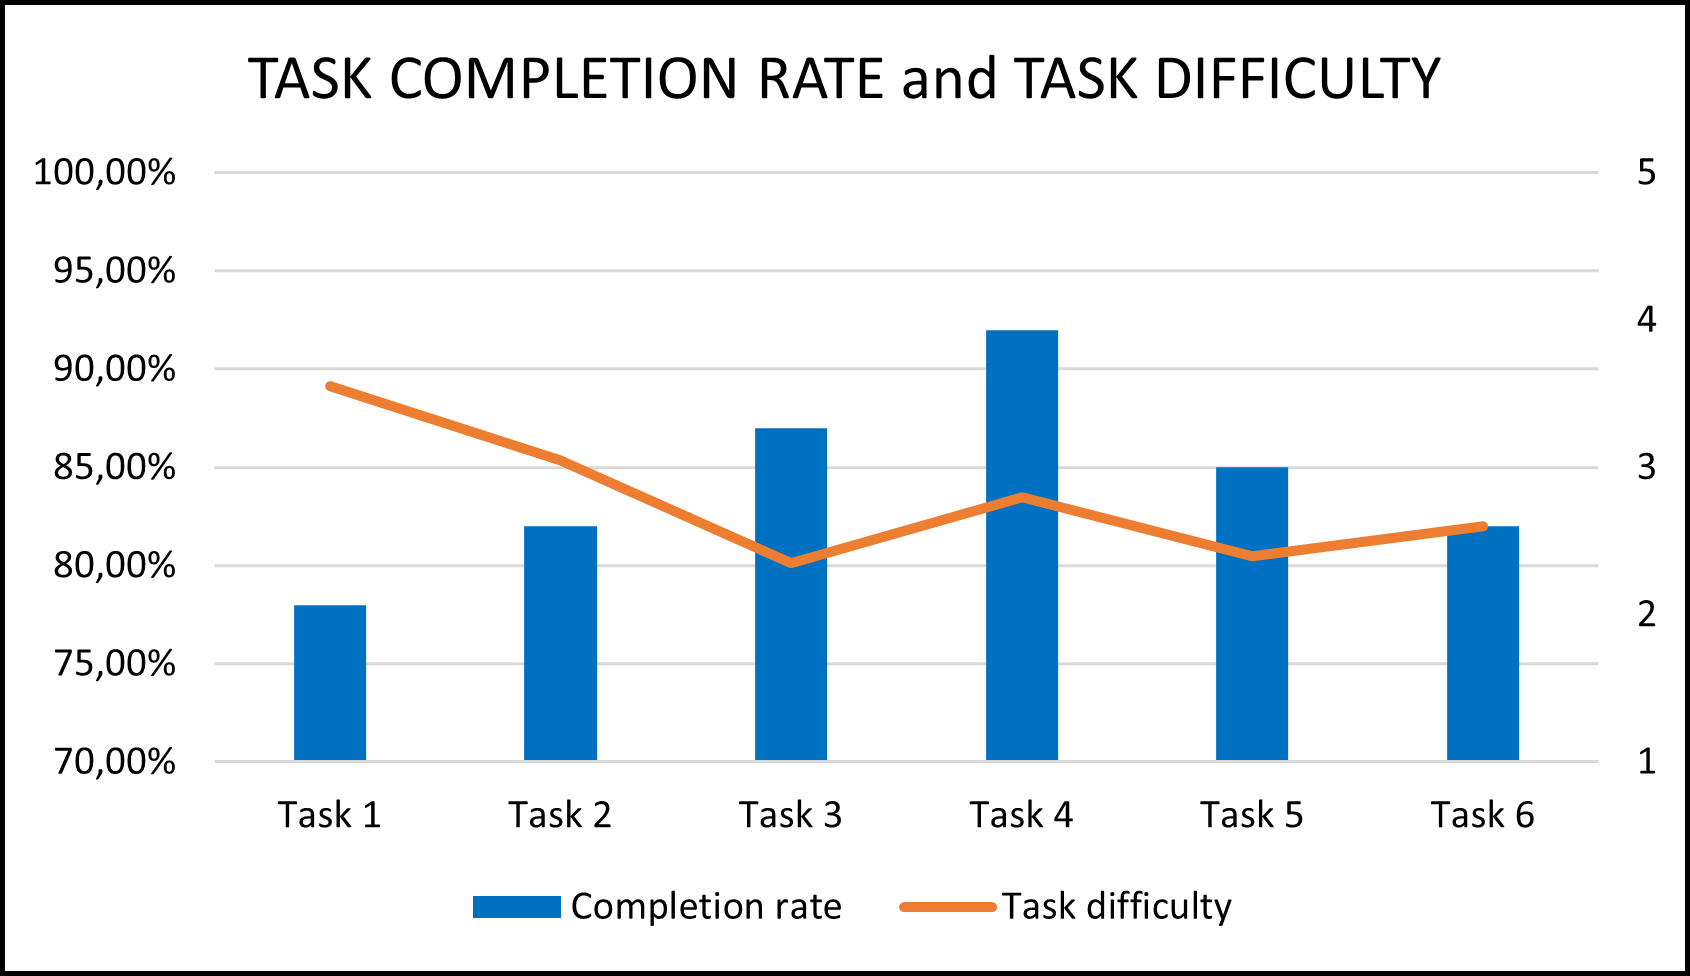
\includegraphics[width=\textwidth]{UT_Visual_illustration_1.png}
	\caption{\textit{TASK COMPLETION RATE and TASK DIFFICULTY.}}
	\label{fig:label1}
\end{figure}
\begin{figure}[h]
	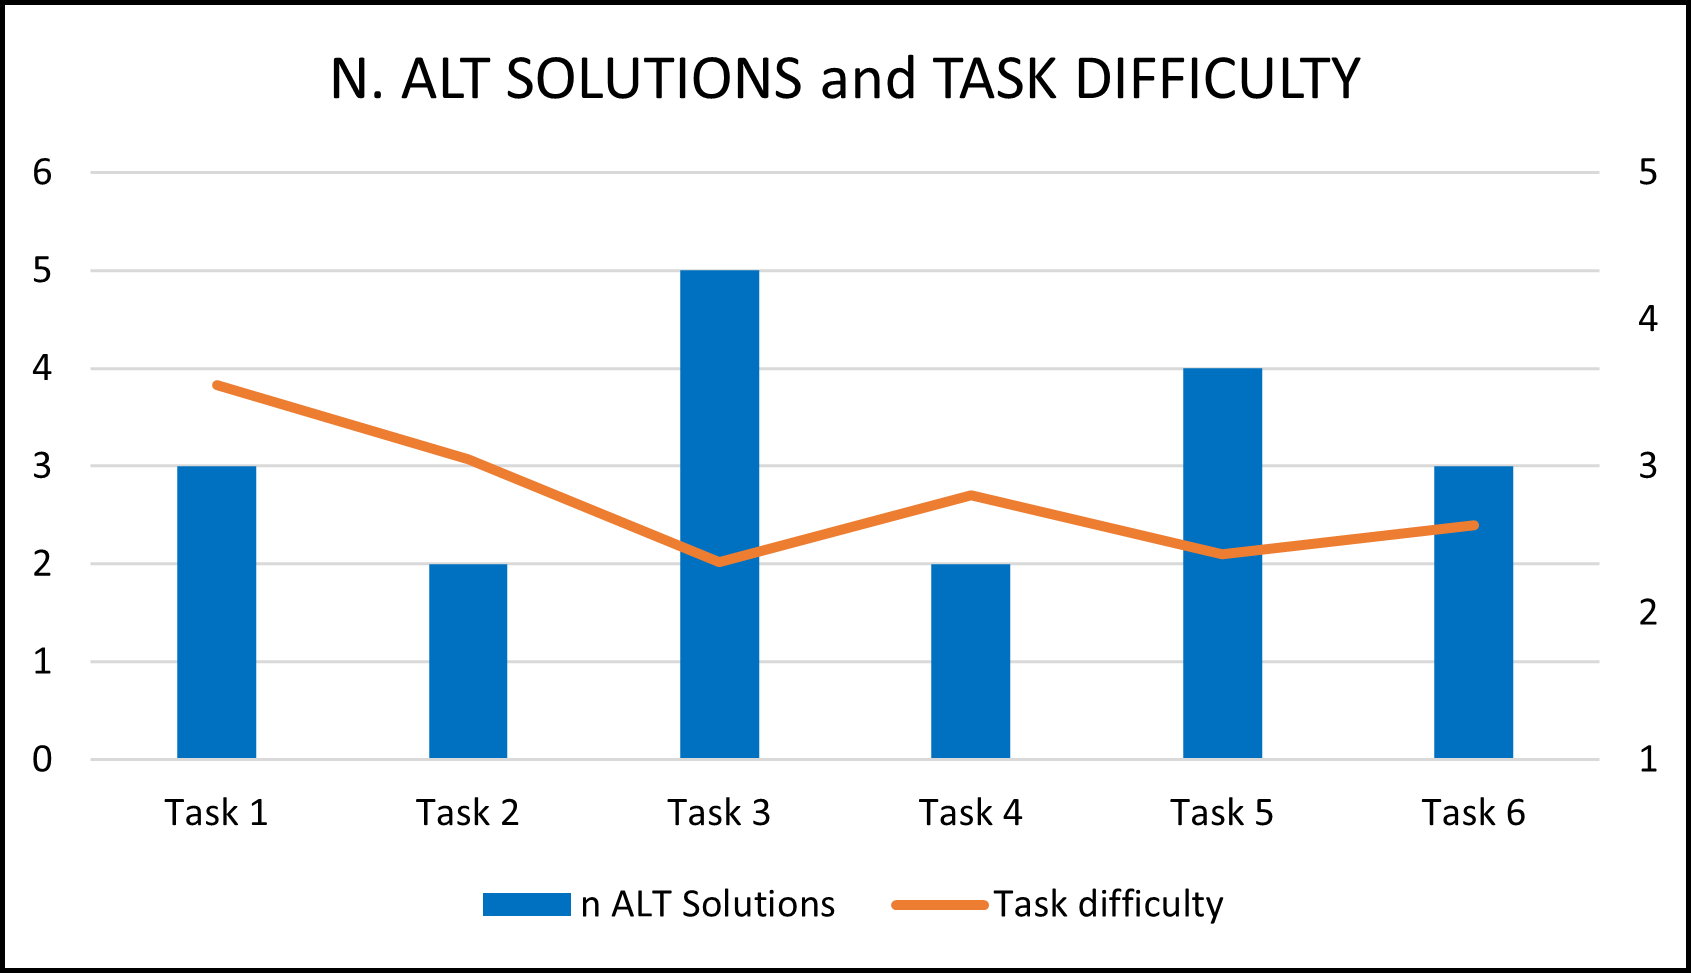
\includegraphics[width=\textwidth]{UT_Visual_illustration_2.png}
	\caption{\textit{N. ALT SOLUTIONS and TASK DIFFICULTY.}}
	\label{fig:label2}
\end{figure}
\begin{figure}[h]
	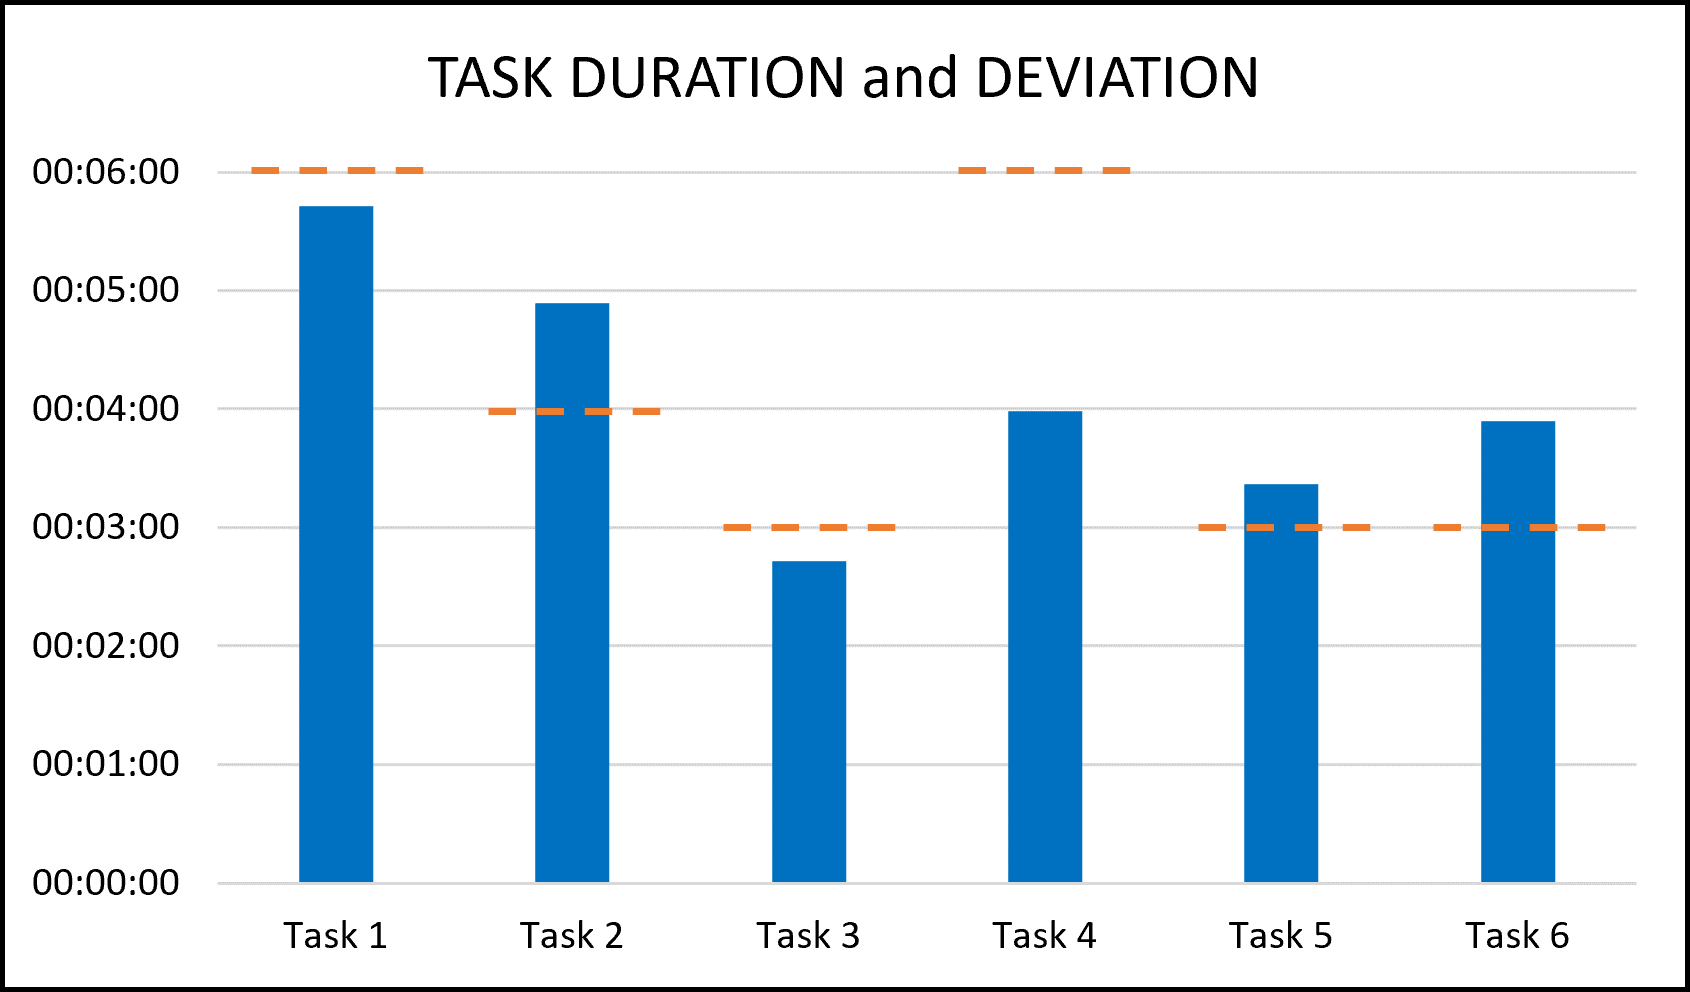
\includegraphics[width=\textwidth]{UT_Visual_illustration_3.png}
	\caption{\textit{TASK DURATION and DEVIATION.}}
	\label{fig:label3}
\end{figure}
\begin{figure}[h]
	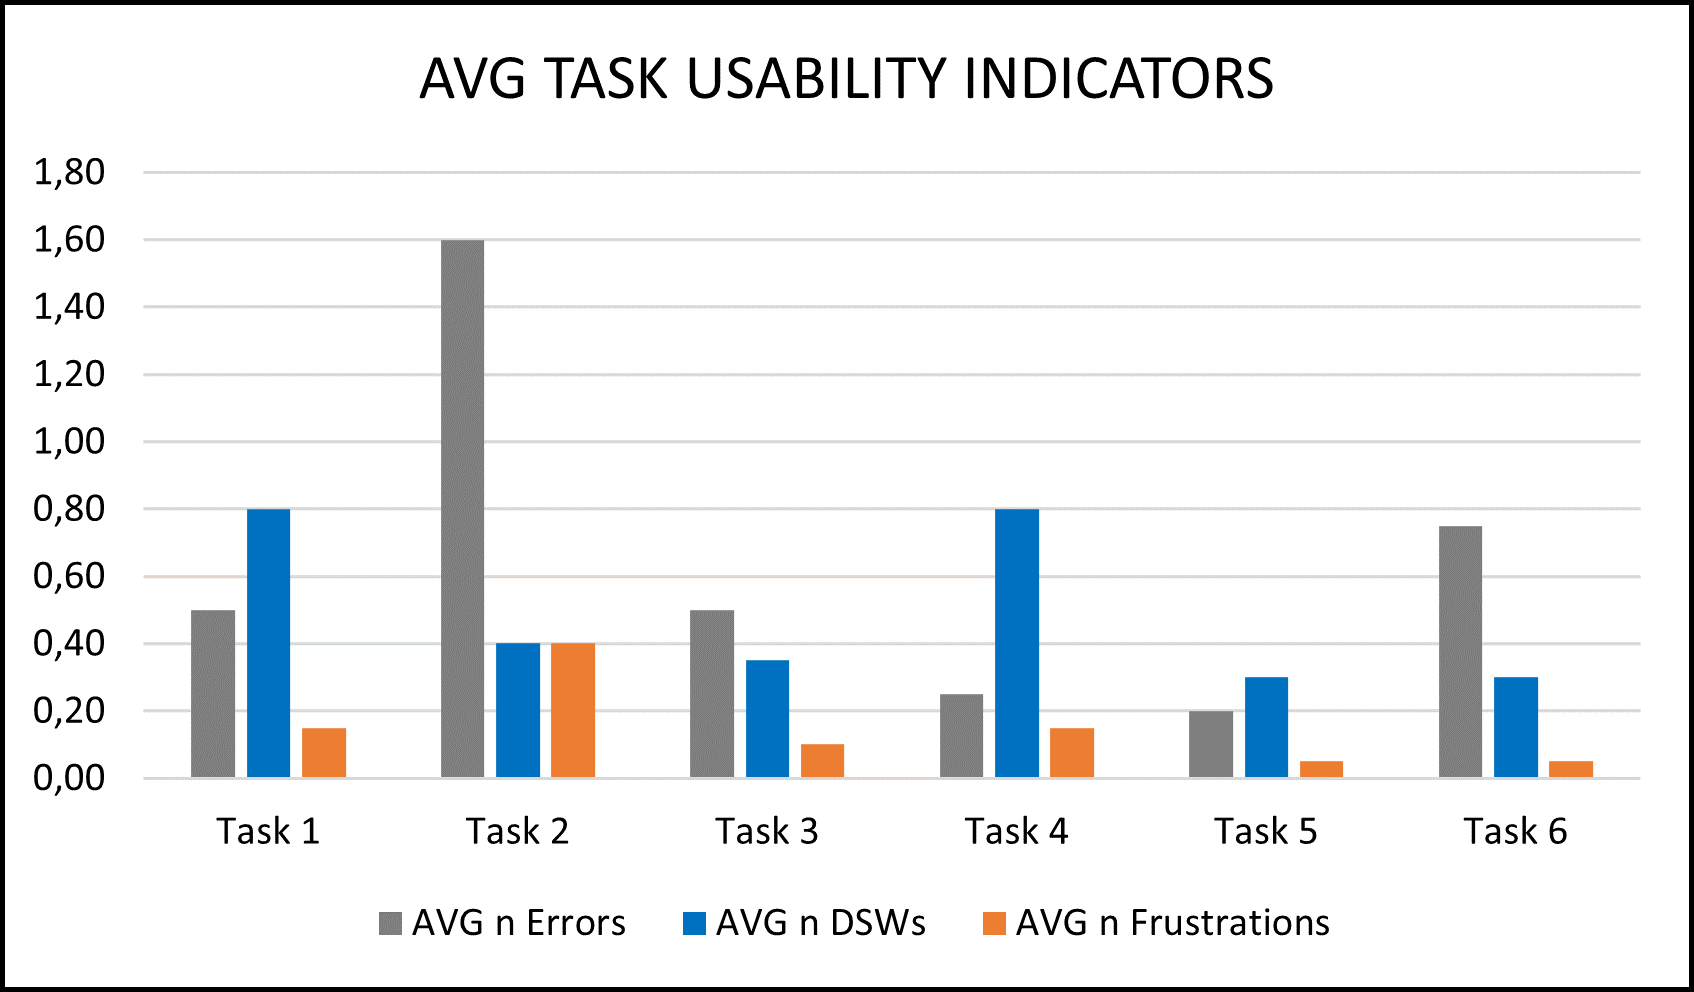
\includegraphics[width=\textwidth]{UT_Visual_illustration_4.png}
	\caption{\textit{AVG TASK USABILITY INDICATORS.}}
	\label{fig:label4}
\end{figure}
\begin{figure}[h]
	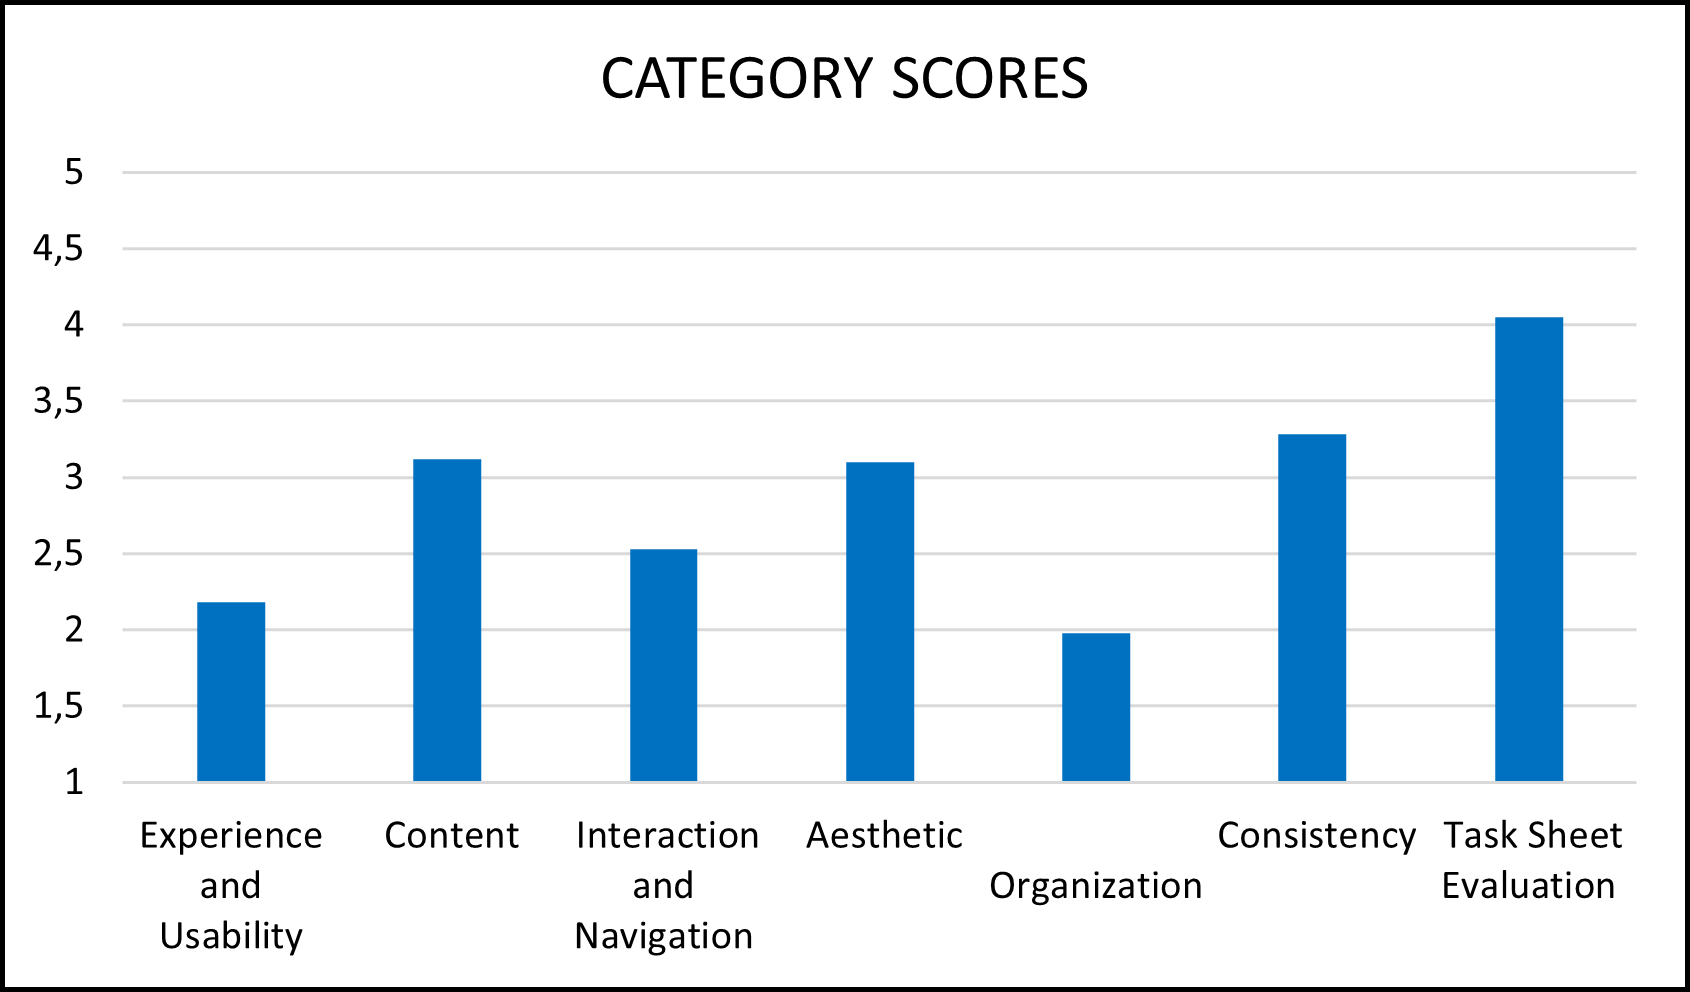
\includegraphics[width=\textwidth]{UT_Visual_illustration_5.png}
	\caption{\textit{CATEGORY SCORES.}}
	\label{fig:label5}
\end{figure}
\begin{figure}[h]
	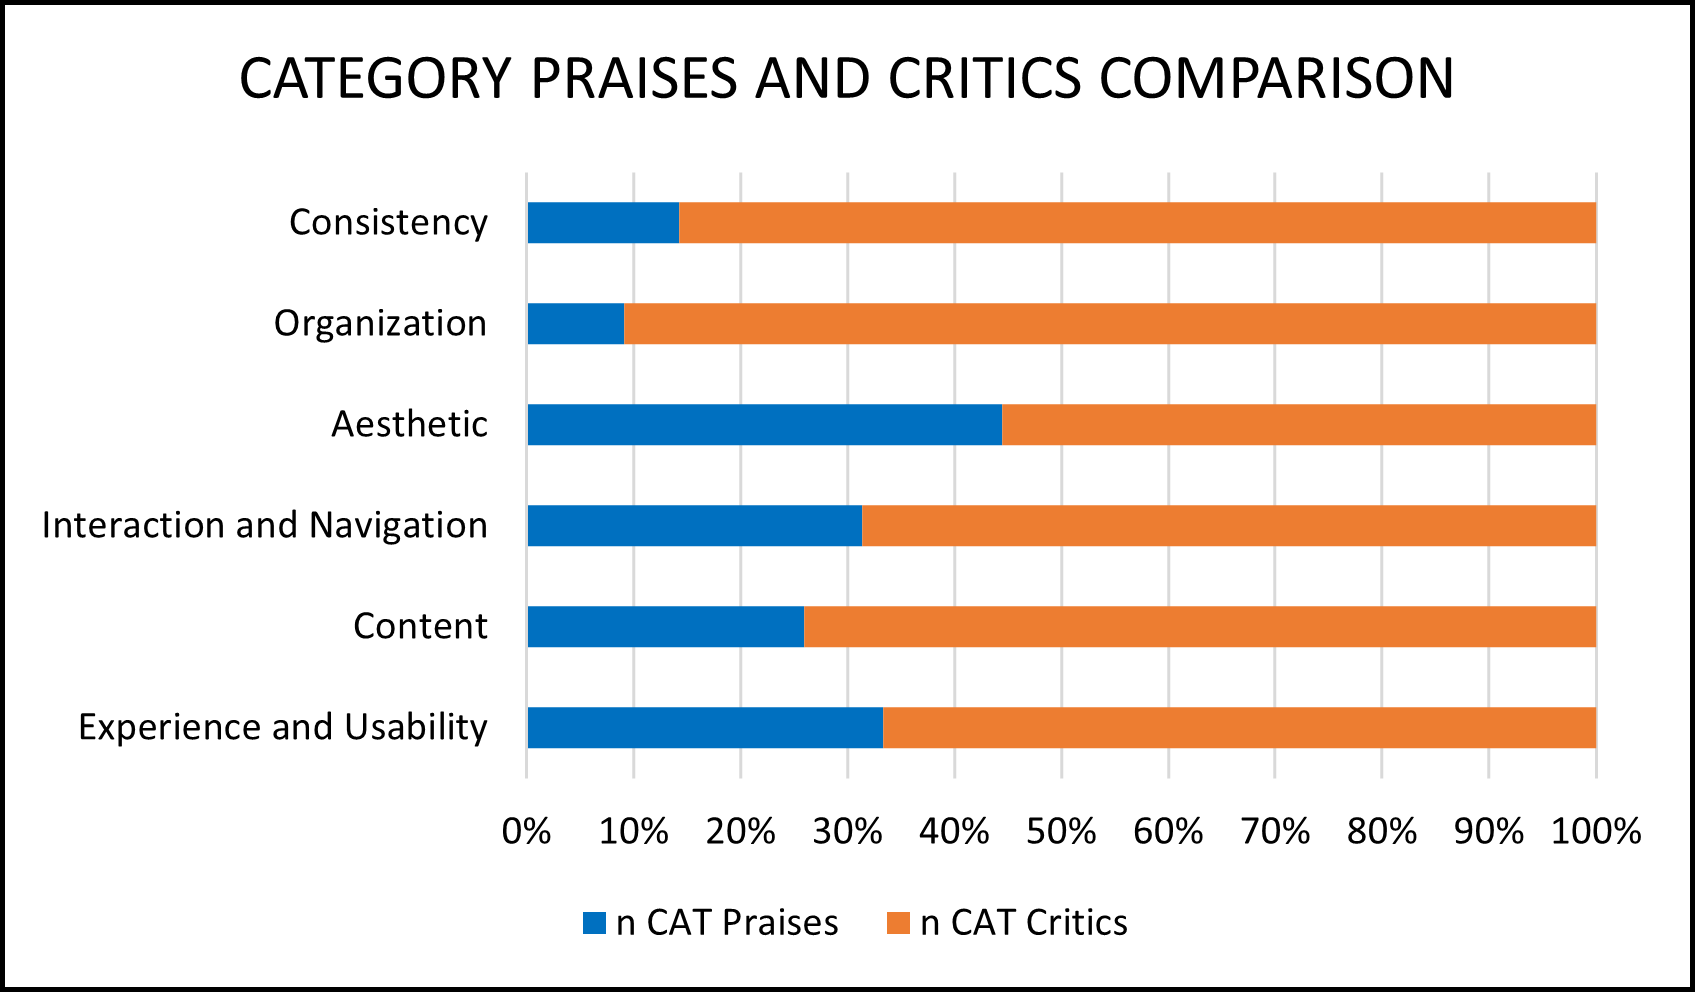
\includegraphics[width=\textwidth]{UT_Visual_illustration_6.png}
	\caption{\textit{CATEGORY PRAISES AND CRITICS COMPARISON.}}
	\label{fig:label6}
\end{figure}
\begin{figure}[h]
	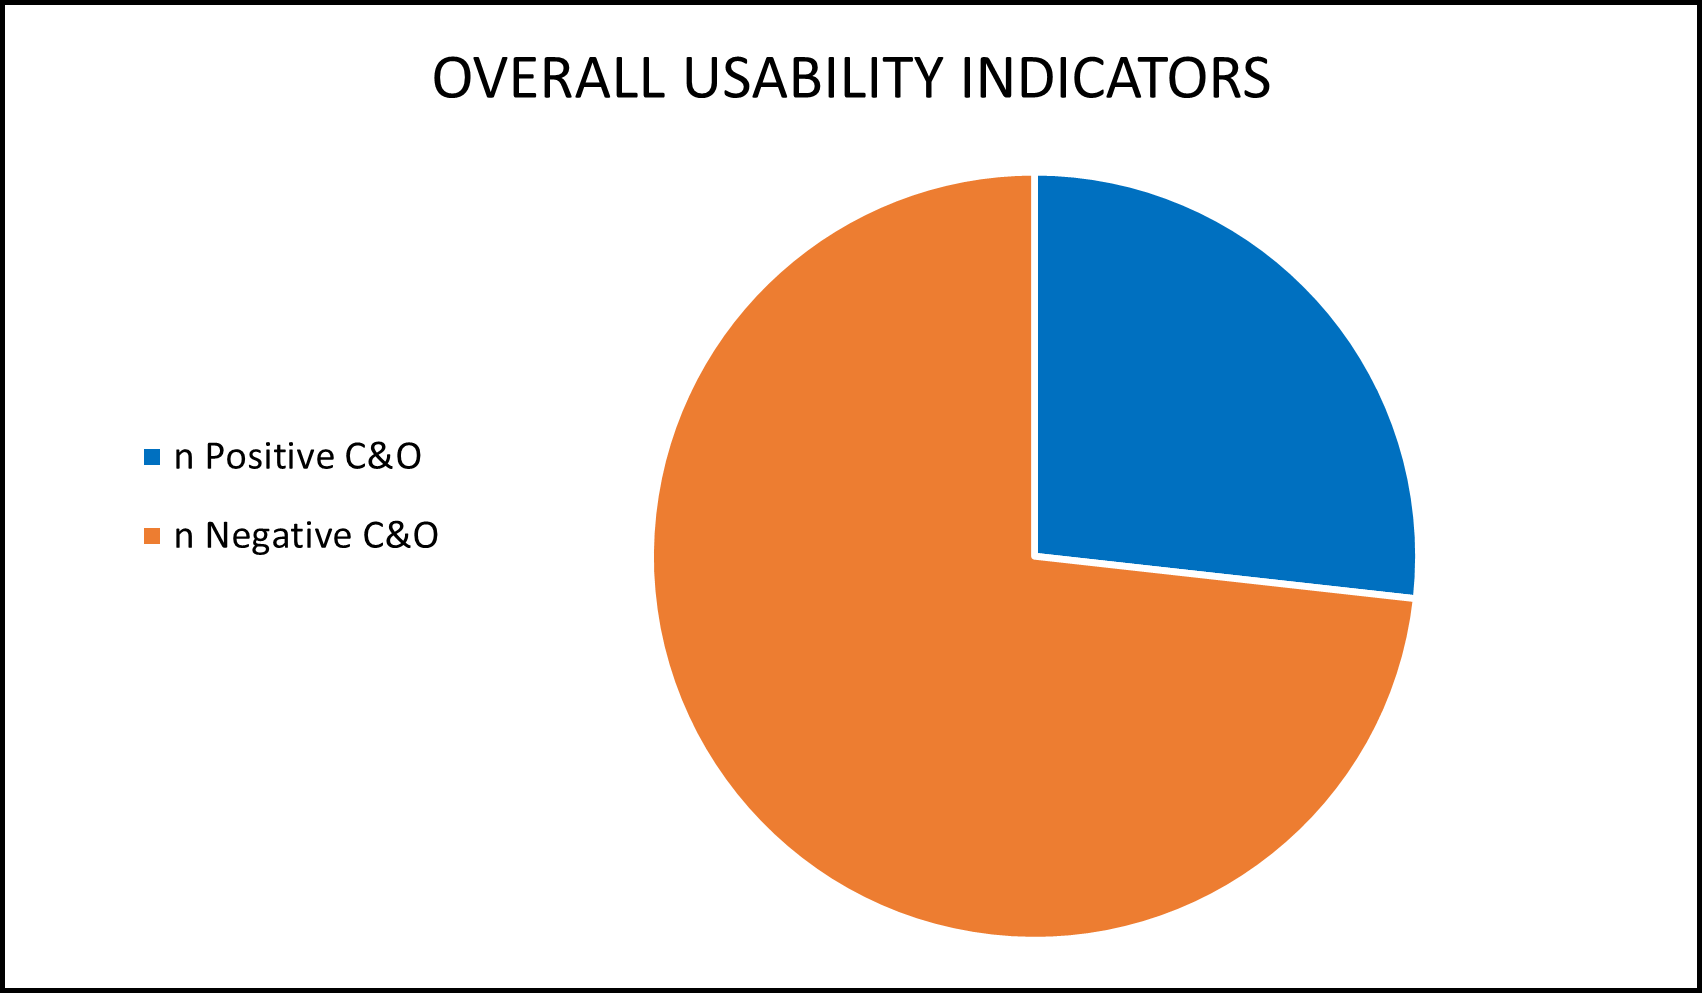
\includegraphics[width=\textwidth]{UT_Visual_illustration_7.png}
	\caption{\textit{OVERALL USABILITY INDICATORS.}}
	\label{fig:label7}
\end{figure}
